\section{Results} \label{results}

We estimated the contributions of recombination and context to the variance in SNV density using data from the Ensembl variation database \citep{Cunningham2015}. The SNV density for a sequence is defined as the number of qualified SNVs in the sequence divided by the sequence length. Only 1KG Project \citep{Auton2015} variants were considered in the interests of consistency in SNV discovery. The point mutation direction from which a SNV was derived was inferred using the ancestral nucleotide state as recorded in Ensembl. Counts of filtered variants used by chromosome are shown at Supplementary Table \ref{tab:supp-counts}.

\subsubsection*{Effect of recombination on SNV density}

We evaluated the relationship between recombination and SNV density using linear regression. Our aim was to recover the slope and intercept parameters from which other quantities of interest can be inferred. The slope parameter gives us the increase in SNV density for a given increase in recombination rate. In particular, a positive slope parameter indicates a positive effect of recombination on SNV density and hence mutation. The intercept parameter is the value of SNV density corresponding to a recombination rate of zero under the model. The estimated variance in SNV density due to recombination, which we denote by $\hat{\sigma }^2_{rec}$, is calculated as the difference between the total variance in SNV density and the sum of squares of the residuals.  The ratio of this quantity to total variance in SNV rate is the proportion of variance in SNV rate attributable to recombination. This ratio is the standard metric $R^2$ (coefficient of determination), which measures the fit of a linear model in terms of explained variance in the observed data.

In modelling the influence of recombination, we used a partitioning of the genome into 10-kb segments for which average sex-averaged recombination rates were available \citep{Kong_2010}. These rates are normalized relative to the average genetic distance over all of the 10-kb bins of 0.0116 centimorgans. SNV densities were derived from the number of SNVs in a segment. 

We began by fitting an ordinary least squares linear regression (OLSLR) model to the data. Use of an OLSLR model for inference requires residuals to be mutually independent, in particular that there is no correlation between adjacent bins along the genome (spatial auto-correlation). By analysing the residuals from an OLSLR model we identified a high level of auto-correlation (see Supplementary Figure \ref{fig:autocorrelation}) and determined that they were most appropriately modelled by an ARMA$(p,q)$ model, where $p$ and $q$ are non-negative integers and $p>0$ (see \nameref{methods}) . For each chromosome, we tested a range of ARMA models to find the one with the lowest Akaike Information Criterion (AIC) score for the data. The slope, intercept and ARMA error parameters were simultaneously estimated using a Bayesian Markov Chain Monte Carlo (MCMC) approach (see \nameref{methods}), obviating the need for iterative ``adjustment'' steps. 

The above process was applied to all chromosomes individually. The estimates for variance in SNV rate due to recombination ($\hat{\sigma }^2_{rec}$) are shown as violin plots in Figure \ref{fig:recomb-violin}. It can be seen that there were some significant differences in the variance estimates for different chromosomes. In particular, chromosomes 9, 15, 16, 17 and 22 show significantly higher levels of variance in SNV density due to recombination. There were also significant differences in estimates of the slope and intercept parameters (see Supplementary Table \ref{tab:supp-recomb}). These differences between chromosomes precluded estimation of the influence of recombination across the genome as a whole. Specifically, using a model which set the slope and intercept parameters to be common across chromosomes while allowing differing ARMA models and parameters for each chromosome resulted in a y-intercept that was larger than the average SNV density, which is inconsistent with results from individual chromosomes. Modifications of this approach that used the sex-specific recombination maps did not result in any substantial differences (results not shown).

\begin{figure*}[h!]
\begin{center}
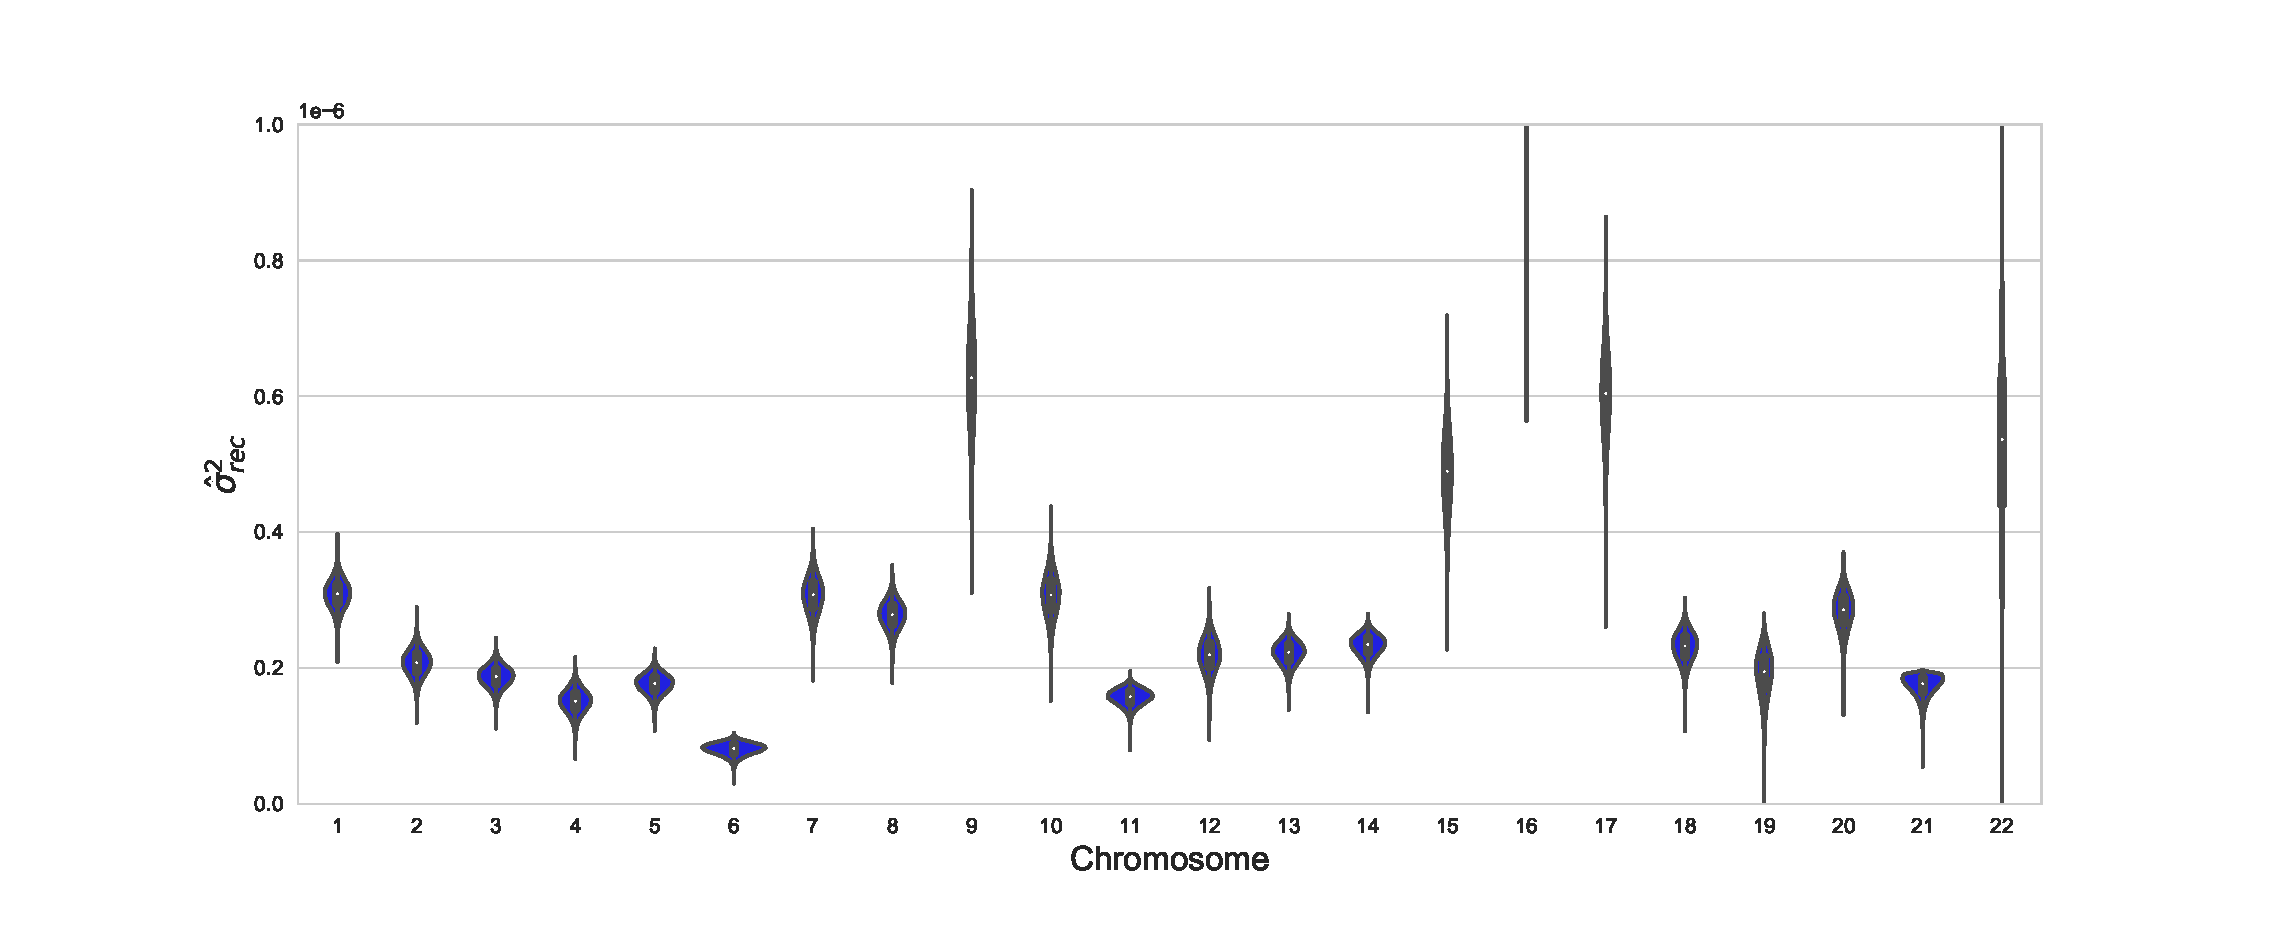
\includegraphics[width=1.0\textwidth]{figs/violin_plot_sexav_mono.eps}
\caption{Estimated variance in SNV density attributable to recombination by chromosome. The variances ($\sigma^2_{rec}$) are estimated by fitting a linear model to each chromosome, with residuals modelled by an ARMA(p,q) model optimised for each chromosome. The variance due to recombination is the difference between total variance and the variance not explained by the model.}
\label{fig:recomb-violin}
\end{center}
\end{figure*}

Estimates for the slope (change in SNV density per centimorgan) provided strong evidence for a positive effect of recombination on SNV density across all chromosomes. The estimates ranged from 0.0061 for chromosome 4 to 0.0092 for chromosome 14 (see Supplementary Table \ref{tab:supp-recomb}). The corresponding 95\% credibility intervals (hereafter CI) of these estimates were 0.0044-0.0078 and 0.0057-0.010 respectively. For all chromosomes tested, the posterior probabilities that the slope was $\leq 0$ were $\leq 10^{-3}$ (estimated from the MCMC variates).

In the linear model, the y-intercept represents the predicted SNV density for a recombination rate of zero. Estimates for the y-intercept ranged from 0.0251 (95\% CI of 0.0246-0.0255) for chromosome 1 to 0.0285 (95\% CI of 0.0257-0.0313) for chromosome 16. The difference between the mean SNV density and the y-intercept parameter is more significant as it represents the difference between the average observed SNV density calculated and the observed data and the SNV density predicted for a recombination rate of 0. That is, this difference measures the part of the SNV density that can be attributed  to recombination under the model. Dividing the difference by mean SNV density gives the proportion of SNVs that can be attributed to recombination ($\hat\rho$, \nameref{methods}). This quantity varied between 0.24\% for chromosome 4 and 0.59\% for chromosome 8. 

We also examined the extent to which the effect of recombination on SNV density differed for the 12 point mutations directions for each chromosome. As an example, results for chromosome 1 are shown in Table \ref{tab:recombination_mutation_types}. We accepted that recombination has had a positive effect on mutation when the posterior probability that the slope was less than zero was found to be less than 0.05. On this basis, the mutations for which recombination influenced mutation in Chromosome 1 comprise all four transitions 
(C\textrightarrow T, T\textrightarrow C, A\textrightarrow G, G\textrightarrow A) and the N\textrightarrow S transversions C\textrightarrow G, G\textrightarrow C, T\textrightarrow G and A\textrightarrow C.

For SNVs derived from transition mutations, evidence for an association with recombination rate was consistent across all chromosomes (Figure \ref{fig:rcomb-heatmap} and Supplementary Table \ref{supp_recombination_chromosomes}). This was not the case for the transversion mutations. For SNVs derived from transversions, evidence of an influence of recombination ranged from inconsistent to none. For instance, for transversions to G/C, the posterior probabilities for most chromosomes met our 0.05 threshold. In contrast, there was no evidence of an influence of recombination on transversions to A/T for most chromosomes. Additionally, if a mutation type appears to be influenced by recombination, so does its strand-symmetric counterpart. However, the values for variance due to recombination for a mutation and its strand-symmetric counterpart, while of similar magnitude, do not necessarily coincide, even using the 95\% CI. For all chromosomes the mutations with the highest variance due to recombination are C\textrightarrow T and G\textrightarrow A, the same as are subject to the CpG effect.

\begin{table}[htp!]
\footnotesize
\caption {\footnotesize Analysis of the linear relationship between recombination rates and SNV densities for chromosome 1 disaggregated by mutation direction. SNV Density' is the SNV density for that mutation direction (conditioned on ancestral allele); `Probability' is the posterior probability that the slope parameter from the linear regression is less than zero; `$\hat{\sigma }^2_{rec}$' is the estimated variance due to recombination and  `Lower CL 95\%' and  `Upper CL 95\%' are the limits of the 95\% credibility interval for $\hat{\sigma }^2_{rec}$.
 } \label{tab:recombination_mutation_types}
\centering
\begin{tabular}{ l c c c c c }
\hline
\bf{Mutation} & \bf{SNV Density} & \bf{Probability} & \bf{$\hat{\sigma }^2_{rec}$} & \bf{Lower CL 95\%} & \bf{Upper CL 95\%} \\
\hline
\hline
C\textrightarrow T &      0.0247 &      0.0000 &                 3.7e-07 &       2.9e-07 &       4.4e-07 \\
G\textrightarrow A &      0.0246 &      0.0000 &                 3.8e-07 &       3.0e-07 &       4.4e-07 \\
T\textrightarrow C &      0.0124 &      0.0000 &                 5.0e-08 &       4.4e-08 &       5.3e-08 \\
A\textrightarrow G &      0.0125 &      0.0000 &                 8.2e-08 &       7.1e-08 &       9.1e-08 \\
C\textrightarrow G &      0.0047 &      0.0004 &                 2.6e-09 &       1.4e-09 &       3.1e-09 \\
G\textrightarrow C &      0.0047 &      0.0022 &                 1.0e-09 &       4.4e-10 &       1.2e-09 \\
T\textrightarrow G &      0.0030 &      0.0109 &                 9.3e-10 &       1.9e-10 &       1.3e-09 \\
A\textrightarrow C &      0.0030 &      0.0168 &                 9.4e-10 &       9.2e-11 &       1.4e-09 \\
T\textrightarrow A &      0.0029 &      0.9472 &                -2.8e-10 &      -9.5e-10 &       1.9e-12 \\
A\textrightarrow T &      0.0029 &      0.3697 &                 9.6e-12 &      -5.6e-10 &       2.3e-10 \\
C\textrightarrow A &      0.0054 &      0.9140 &                -5.3e-10 &      -2.0e-09 &      -1.3e-12 \\
G\textrightarrow T &      0.0054 &      0.9290 &                -8.9e-10 &      -2.8e-09 &       6.2e-11 \\
\hline
\end{tabular}
\\ \raggedright{Since the estimated variance in SNV density due to recombination is calculated as the difference between the total variance in SNV density and the sum of squares of the residuals, it will be negative if the model fit is worse than for a line with zero slope. This is likely to occur when the `Probability' value is significantly greater than zero and we reject the model.}
\end{table}


\begin{figure}[h!]
\begin{center}
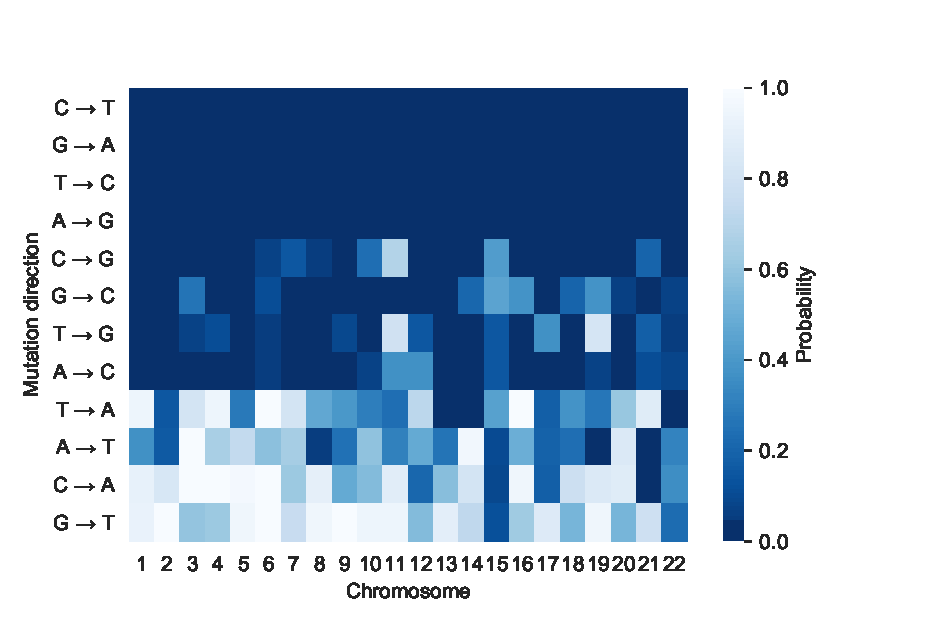
\includegraphics[width=1.0\columnwidth]{figs/heatmap.eps}
\caption{Evidence for the effect of recombination on mutation by mutation direction and chromosome.  `Probability' is the posterior probability that the slope parameter from the linear regression is less than zero. A darker shade indicates a high probability that SNV density has a positive linear relationship with recombination. Cells meeting the 0.05 threshold are in the deepest blue.}
{\label{fig:rcomb-heatmap}}
\end{center}
\end{figure}

\subsubsection*{Variance in SNV density due to context}

In our analysis of variance in SNV density due to context, we restricted ourselves to intronic 1KG Ensembl variants, to reduce confounding due to selection. All SNVs and contexts were oriented with respect to the annotated strand of the gene. For consistency with our assumption that each site has a fixed mutation rate, only biallelic variants separated by $\ge4$ nucleotides from another SNV were considered. Rather than use a conventional sample or plug-in estimator of the average SNV density for each context, we worked with samples from a posterior (beta) distribution to the binomial likelihood function. This allowed us to sample and graph posterior distributions for variance due to context, showing the uncertainty in the parameter estimates (see \nameref{methods}). It also allowed us to calculate the (posterior) probabilities of particular conditions by counting the proportion of MCMC variates satisfying the condition.

To evaluate the relationship between sequence context and the probability of a SNV requires further definition of SNV density. For a specific sequence context of size $k$ (including the middle position), there are $4^k$ distinct contexts (hereafter $k$-mers). To illustrate calculation of SNV density, consider the 3-mer ACA. We estimated the SNV density for ACA as the number of occurrences of ACA for which the middle position had an SNV divided by the total number of occurrences of the $k$-mer ACA. This can be further partitioned into the different point mutations from C. The estimated variance attributable to sequence context of size $k$, which we denote by $\hat{\sigma }^2_k$, is thus the variance computed across all $4^k$ such densities (see \nameref{methods}).

The value of $\hat{\sigma }^2_k$ for $k=$ 1, 3, 5 and 7 is shown by the blue bars in Figure \ref{fig:context-var} for 1-mers to 7-mers. The case of $k=1$ shows variance conditioned solely on ancestral base. We necessarily observe an increase in variance with increasing $k$, but the increments diminish markedly after 3. It is noteworthy that the variance due to the central base alone only comprises $\sim12\%$ of the variance due to 3-mers. The total variance due to 7-mers is $\sim35\%$ greater than that due to 3-mers. Variance in SNV density calculated in this way includes the influence of the central mutating base itself and the interaction between that central mutating base and its neighbourhood. To investigate the relative influence of these elements further, we show, using the brown bars, the values of $\hat{\sigma }^2_k$ marginalised over the central base (Figure \ref{fig:context-var}). That is, we evaluated the influence of the flanking nucleotides alone, by pooling counts of variants and $k$-mers which share the same central base and calculating the variance of the SNV frequencies for the bins formed in this way. We see that while these values are much lower than the unmarginalized values, the relative magnitude of the increments from 3-mer to 5-mer and from 5-mer to 7-mer are larger. We can conclude that the greater part of the unmarginalized variance due to 3-mers is explained not by the independent actions either of the central base or of the flanking bases, but by the interaction of the central base with its immediately adjacent neighbours. Furthermore, this interaction between a mutating base and its immediate neighbours is the largest contribution to variance for all values of $k$ considered. As would be expected,  a large component of this is due to the CpG effect (including its strand-symmetric counterpart) which we estimated as 0.00028, $\sim$ 54\% of the variance due to 7-mers.

%See 'Variance due to context across kmers (incl. central allele).ipynb'
\begin{figure}[h!]
\begin{center}
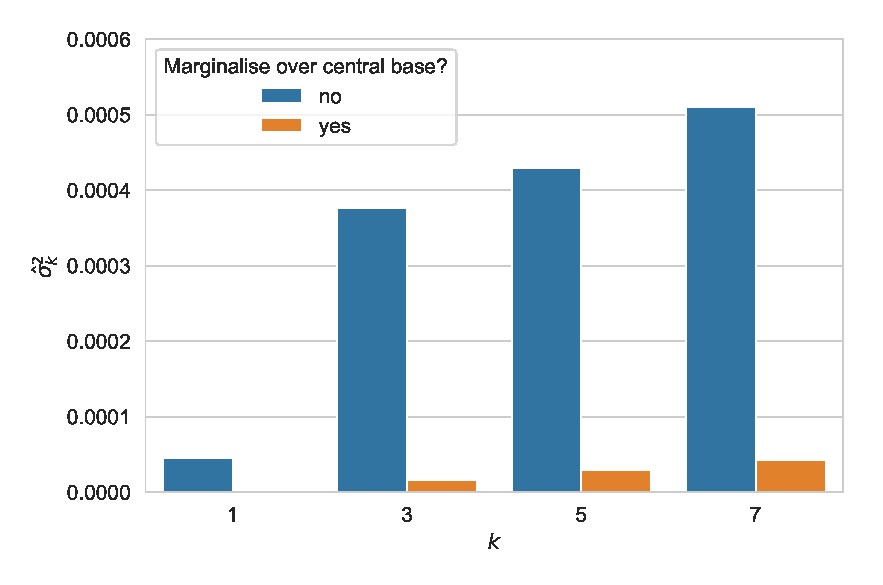
\includegraphics[width=0.75\columnwidth]{figs/context-var.eps}
\caption{The interaction between a mutating base and its neighbourhood dominates variance in SNV density. The component of $\hat\sigma^2_k$ attributable to neighbourhood alone (i.e. marginalised over the central base) is shown in tan. This contrasts with the full value of $\hat\sigma^2_k$ (shown in blue), which includes the interaction between a mutating base and its neighbourhood.}
{\label{fig:context-var}}
\end{center}
\end{figure}

We also analysed the variance due to context for each of the point mutations separately. The results are shown in Figure \ref{fig:context-var-individual} as posterior distributions for the variance due to context. (Values for the posterior mean are shown at Supplementary Table \ref{tab:supp_context}.) The increment in variance from 5-mer to 7-mer is greater than or approximately equal to that from 3-mer to 5-mer for all  point mutations, with the exceptions of T\textrightarrow C / A\textrightarrow G transitions. In the case of transversions, the variance due to 7-mers is approximately two to three times that due to 3-mers. The strong relative influence of 7-mers and 5-mers for transversions may appear to be at odds with the results aggregated over point mutations (Figure \ref{fig:context-var}). However, since Figure \ref{fig:context-var-individual} considers each point mutation separately, the central or `from' base is fixed and the interaction between the central base and its immediate neighbours does not make a contribution. Thus the impact of increasing $k$ is more similar to that of the marginalised quantities (Figure \ref{fig:context-var}).

%\vskip 0.4in
\begin{figure*}[]
\begin{center}
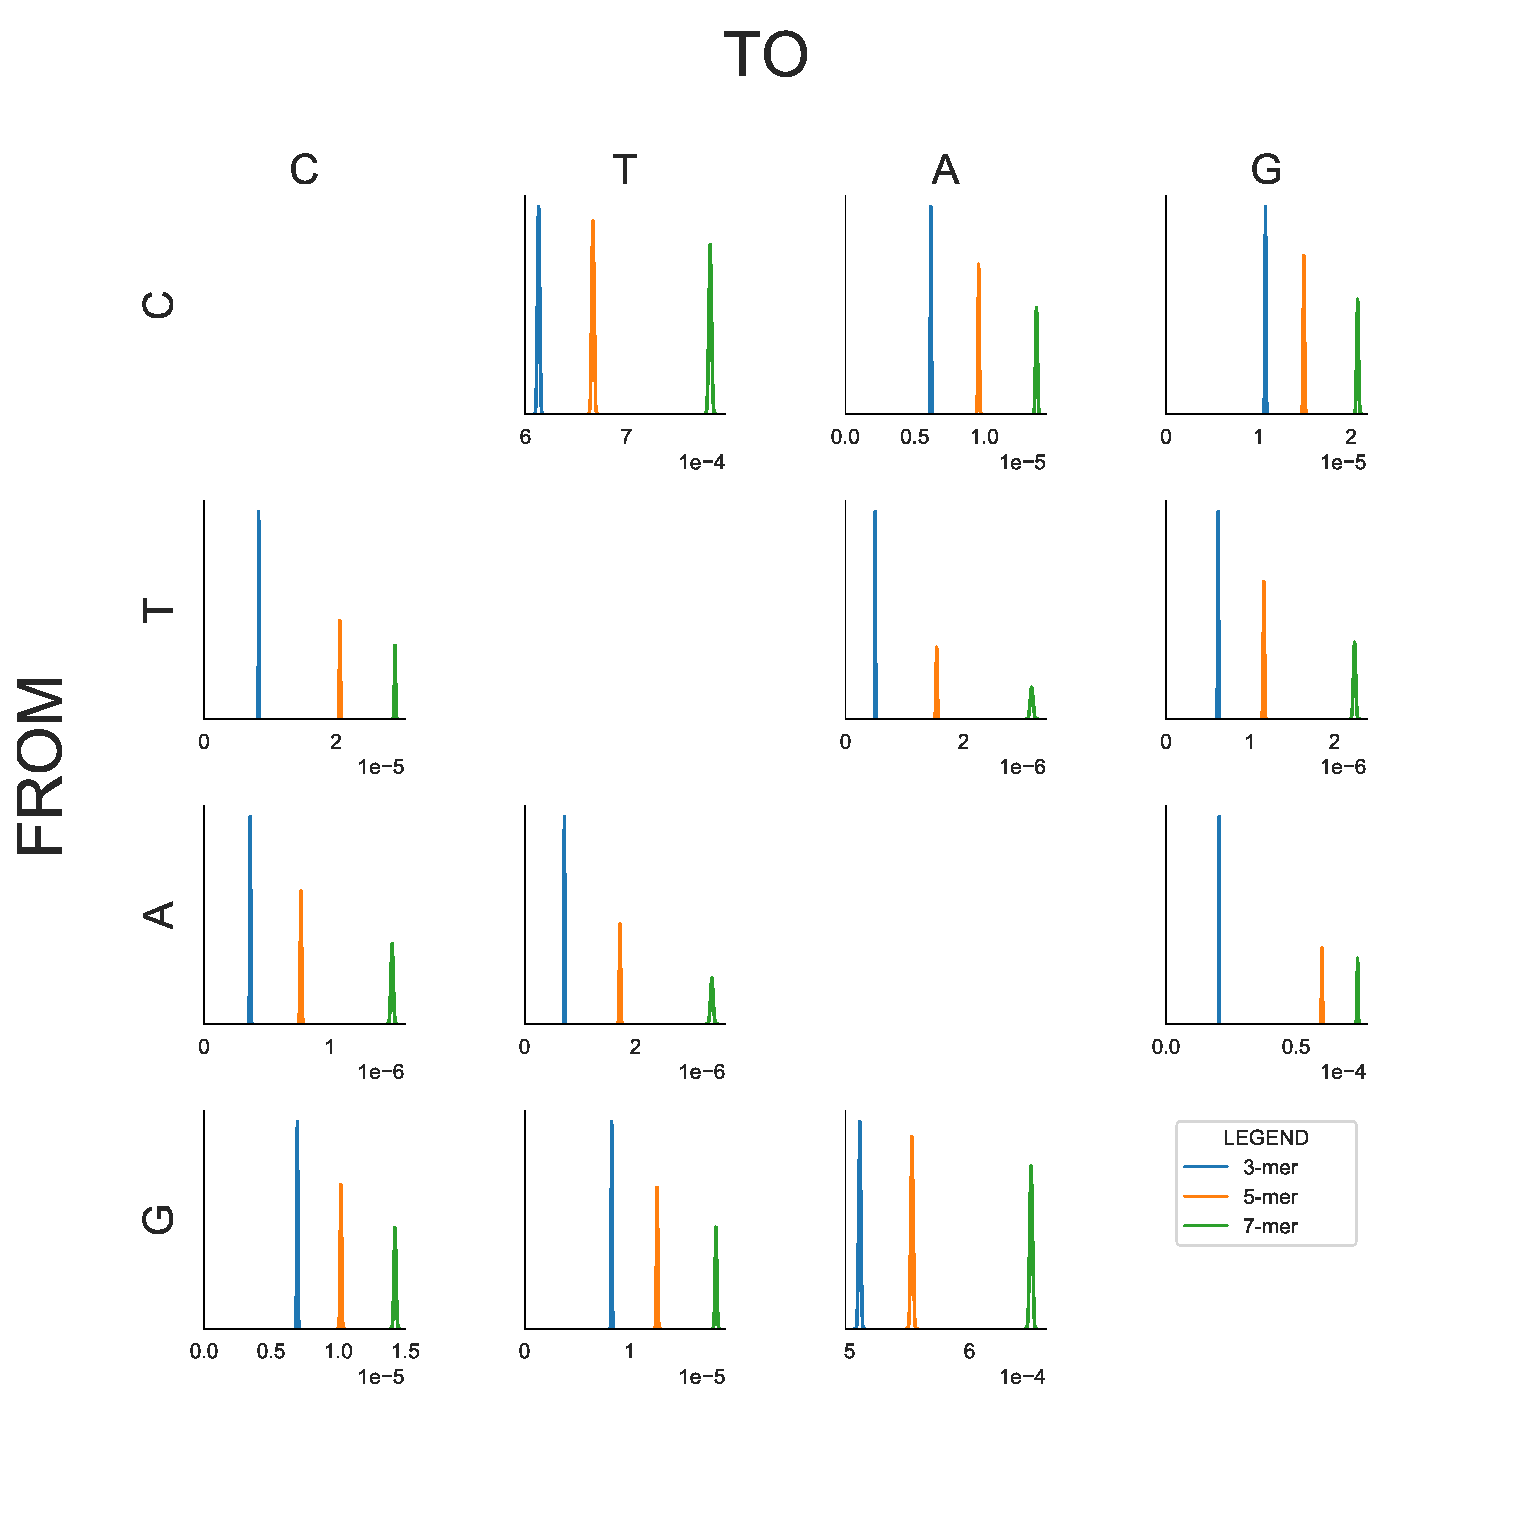
\includegraphics[width=1.0\textwidth]{figs/context-var-individual_200.eps}
\caption{Posterior distributions of the variance of SNV density (x-axis) conditioned on 3-mer, 5-mer and 7-mer contexts for each of 12 mutation profiles. The Row/Column labels correspond to the~\emph{from} and~\emph{to} nucleotides. Note that the x-axes ($\hat\sigma^2_k (a \rightarrow b)$, estimated variance due to context) and y-axes (probability density) scales vary between plots. In particular the x-axes for C\textrightarrow T and G\textrightarrow A mutations do not include the origin.}
\label{fig:context-var-individual}
\end{center}
\end{figure*}

Examination of Figure \ref{fig:context-var-individual} suggests that contextual influence does not always operate in a strand-symmetric manner. We investigated this further by plotting intronic mutations together with their strand-complements for the 7-mer case (Figure \ref{fig:context-sym-intronic-a}). This demonstrates evidence of strand-asymmetry for all mutation types. This was especially marked for T\textrightarrow C / A\textrightarrow G transitions. Our criterion for rejecting strand-symmetry was that the 97.5 percentile of one of a pair of strand-complementary mutations was less than the 2.5 percentile of the other. As a control, we performed a similar analysis for intergenic regions. The results (Figure \ref{fig:context-sym-intronic-b}) are generally consistent with the operation of strand-symmetric processes in intergenic regions. The pair of mutations G\textrightarrow T and C\textrightarrow A appear to be strand-asymmetric by our criterion and may be an exception or an artefact.

\begin{figure*}[]
\begin{subfigure} {1.0\textwidth}
\begin{center}
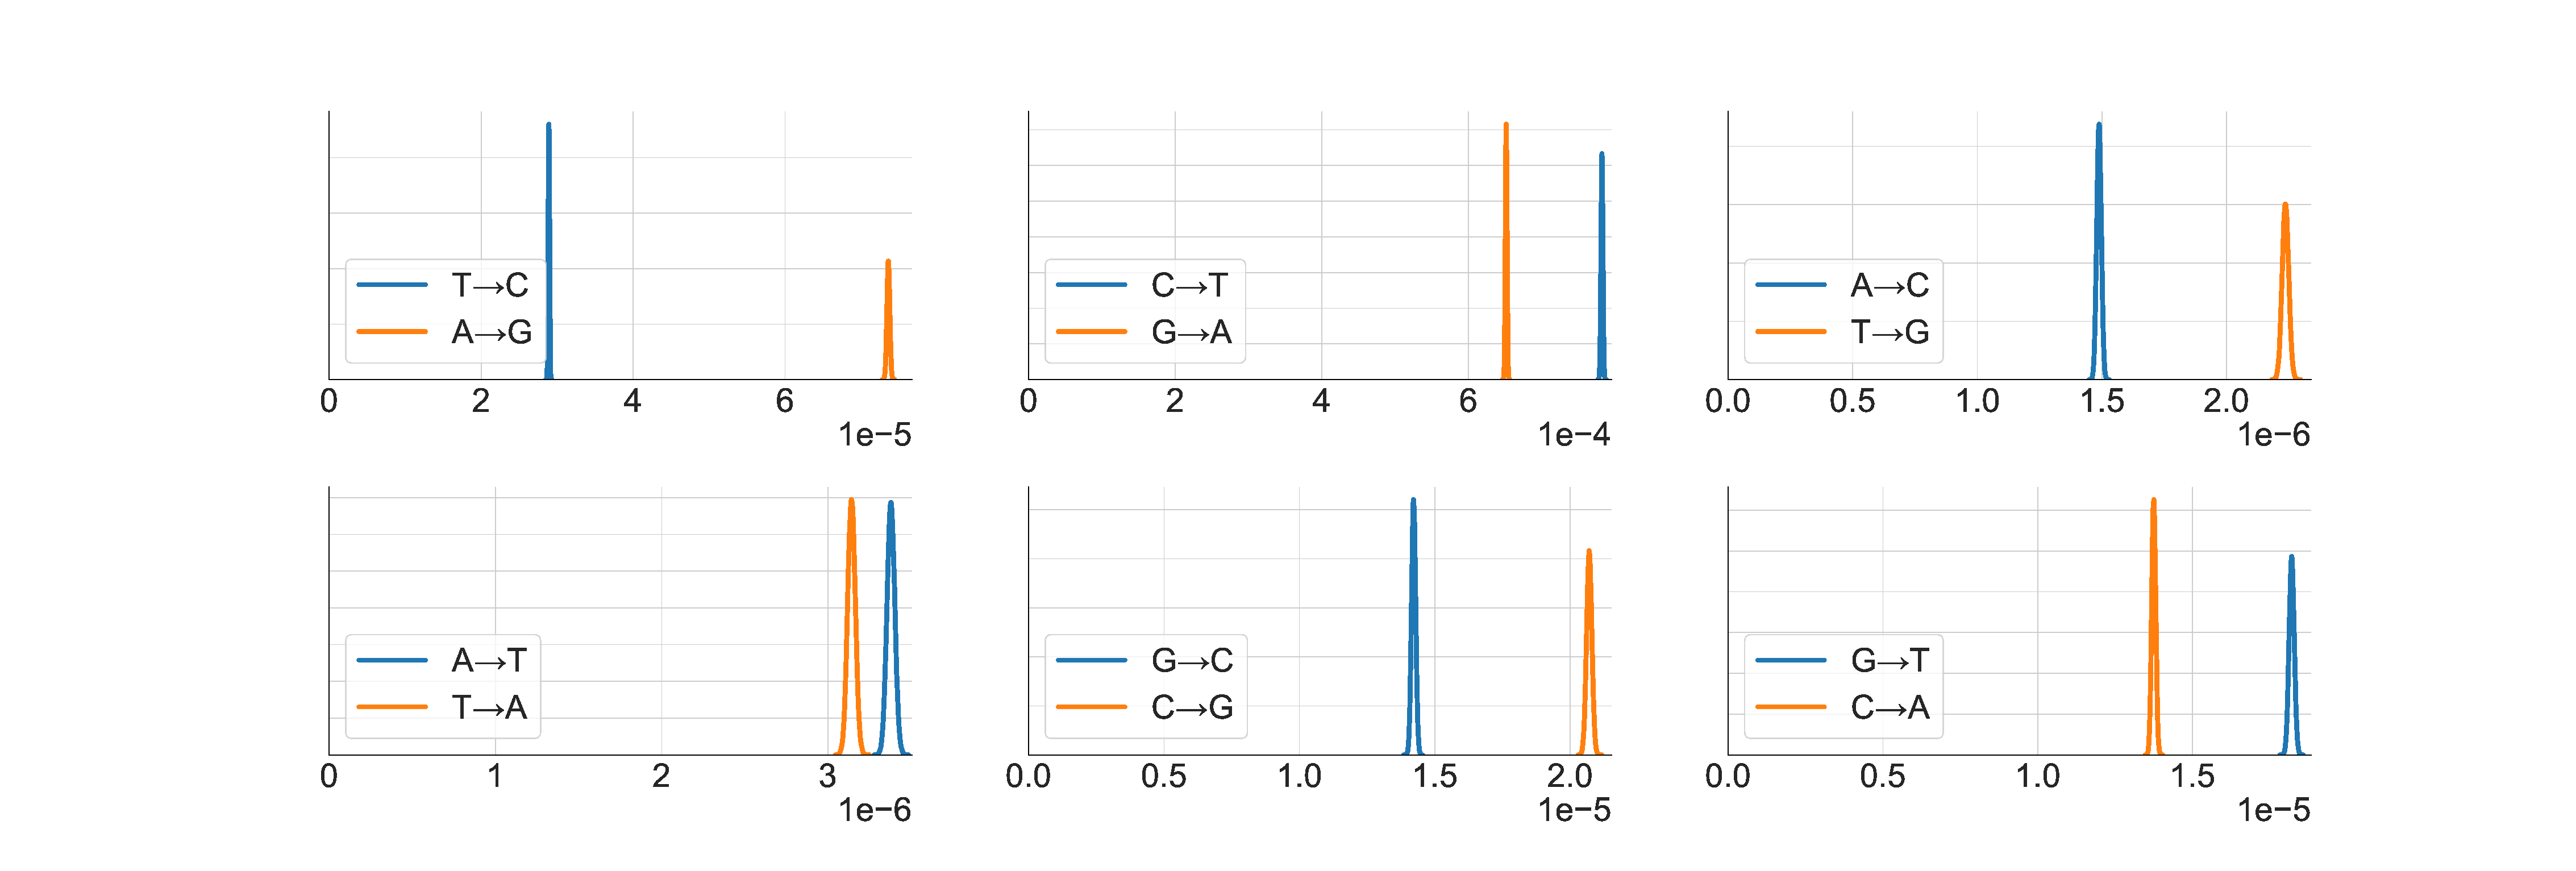
\includegraphics[width=0.95\textwidth, keepaspectratio]{figs/fig_ss_all_a.eps}
\caption 
{\label{fig:context-sym-intronic-a}}
\end{center}
\end{subfigure}
\begin{subfigure}{1.0\textwidth}
\begin{center}
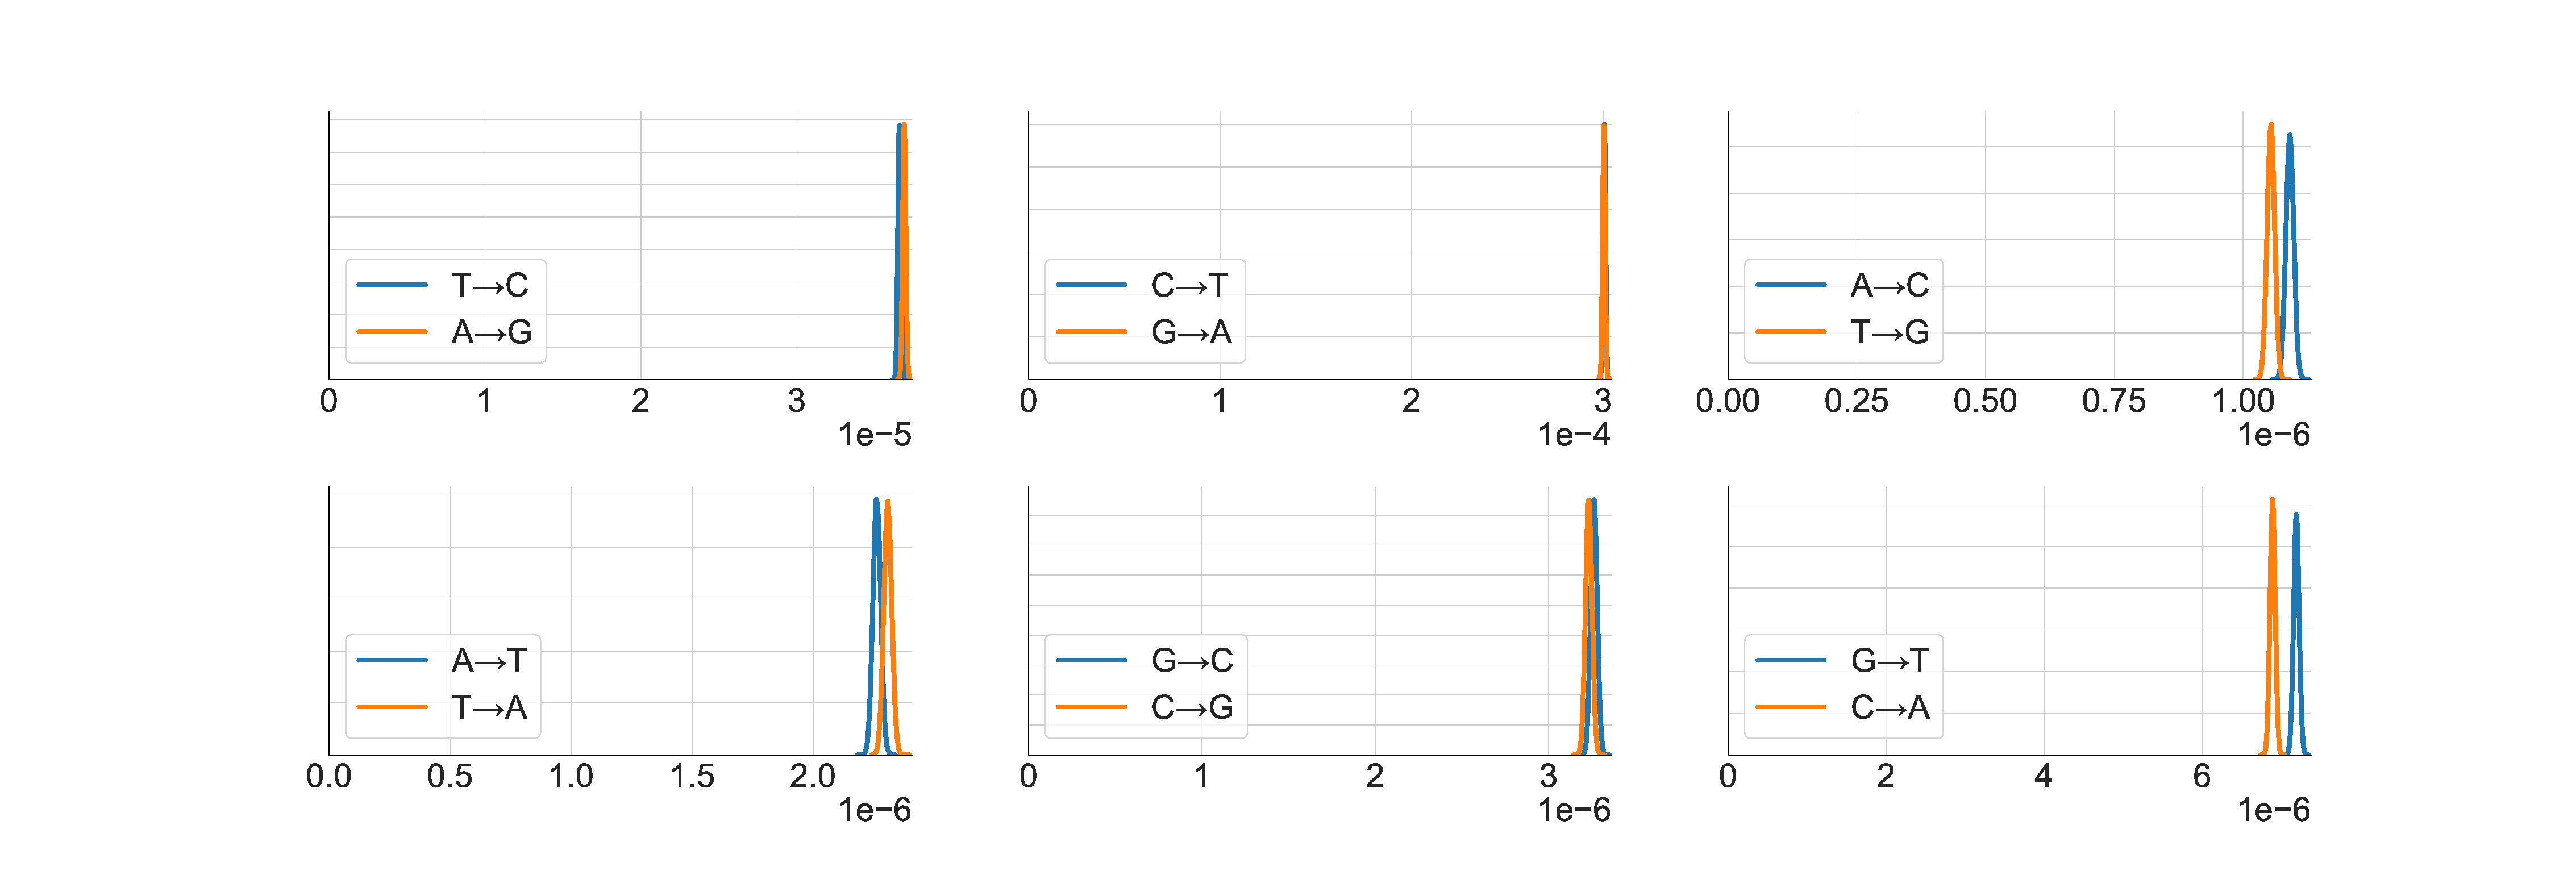
\includegraphics[width=0.95\textwidth, keepaspectratio]{figs/fig_ss_all_b.eps}
\caption 
{\label{fig:context-sym-intronic-b}}
\end{center}
\end{subfigure}
\caption{Variance in SNV density for specific mutation directions is strand-asymmetric for intronic regions, but strand-symmetric for intergenic regions. We show posterior distributions of $\hat{\sigma}_7^2$ for each of the 12 mutation directions (x-axis), with strand-symmetric pairs shown on the same axes. The y-axes show probability density. (a) Intronic regions. (b) Intergenic regions.}
\end{figure*}